\documentclass[10pt,a4paper]{article}
\usepackage[utf8]{inputenc}
\usepackage{amsmath}
\usepackage{amsfonts}
\usepackage{amssymb}
\usepackage{listings}
\usepackage{graphicx}
\usepackage{hyperref}

\newcommand{\CC}{C\nolinebreak\hspace{-.05em}\raisebox{.4ex}{\tiny\bf +}\nolinebreak\hspace{-.10em}\raisebox{.4ex}{\tiny\bf +}}
\def\CC{{C\nolinebreak[4]\hspace{-.05em}\raisebox{.4ex}{\tiny\bf ++}}}
\lstdefinestyle{code}{%
  frame=l, language=bash, numbers=left, numbersep=1em, xleftmargin=2em
}
\lstdefinestyle{codec}{%
  frame=l, language=c++, numbers=left, numbersep=1em, xleftmargin=2em
}
\title{Small Ad-hoc Deep-Learning Library\\{ \normalsize v0.3}}

\date{}
\author{Contact: franck.galpin@interdigital.com}
\begin{document}
\maketitle
\section{Overview}
In this document, we describe SADL (Small Ad-hoc Deep-Learning Library), a header only small \CC library for inference of neural networks. The goals of the library are the following:
\begin{itemize}
\item provide transparent implementation of neural networks based technologies, 
\item ability to assess encoding/decoding time in a common software
\item ability to assess theoretical complexity using library instrumentation
\item ability for proponents to optimize algorithms as it is done in VTM
\item ability to have a matching tool description and source code as during VTM development,
\item ability to crosscheck technology without the need of special environment,
\item reasonable speed performance, no additional overhead
\item possibility to do integer only inference for results repeatability
\item solve licenses and close-source issues, full disclosure of the tools source in accordance with VTM software development policy,
\item no dependency on a particular format, support for multiple DL framework
\item no library dependencies, compatible with VTM/ECM/HM etc.
\end{itemize}
    
\subsection{Constraints}
The following guidelines were used for the development of the library:
\begin{itemize}
\item Dependencies: no (or very few) dependencies, esp. should build from source on any platform
\item Licenses: compatible with JVET software development, typically BSD-3 clauses-clear
\item Architecture: no GPU, no multi-thread, possibly no CPU extension (SIMD)
\item Repeatability: repeatable, platform invariant results (integer inference possible)
\item  Performance: need good performance for practical reasons.
\end{itemize}

\subsection{Summary}
The table below summarize the framework characteristics.
\begin{table}[]
\begin{tabular}{|l|l|}
\hline
Language & Pure C++, header only \\
\hline
Footprint & ~3700 LOC, library ~200kB, no dependency\\
\hline
Optimization & some SIMD at hot spots (best effort)\\
\hline
Compatibility & ONNX file\\
\hline
Layer Supports & constants, add, maxPool, matMul, reshape, ReLU,conv2D, \\
& mul, concat, max, leakyReLU, shape, expand, tranpose, flatten \\
\hline
Type support & float, int32, int16, int8\\
\hline
Quantization & Support adaptive quantizer per layer\\
\hline
License & BSD 3-Clause \\
\hline
\end{tabular}
\end{table}


\section{Quick start}
\subsection{Conversion from ONNX file}
Conversion to the SADL format is done using the script in converter.
\begin{lstlisting}[caption={SADL format conversion},style=code]
python converter/main.py --input_onnx mymodel.onnx \
                         --output mymodel.sadl
\end{lstlisting}

\subsection{Integration inside a program}
\begin{lstlisting}[caption={Model inference in C++},style=codec]
#include <sadl/model.h>

...

tf2cpp::Model<float> model;
std::ifstream file(filename,ios::binary);
if (!model.load(file)) {
    cerr<<"[ERROR] Unable to read model "<<filename<<endl;
    return -1;
}
auto inputs=model.getInputsTemplate();

if (!model.init(inputs)) {
        cerr<<"[ERROR] Pb init"<<endl;
        return -1;
}
...
// fill inputs here
if (!model.apply(inputs)) {
        cerr<<"[ERROR] Pb apply"<<endl;
        return -1;
}
auto output=model.result(); // tensor of the result
\end{lstlisting}

\subsection{Options}
Several build options are available. The macro can be put before the \texttt{\#include <model.h>} in order to control the features availability. All options are available in the file  \texttt{options.h}.

\subsubsection{Optimization options}
Depending on the SIMD level used to build the file, SIMD version of some functions are available.
At the time, the SIMD configuration is not dynamic. In order to choose the SIMD level, the \texttt{\#include <model.h>} directive should be isolated inside a unique cpp file and compile with the desired SIMD option.
The following SIMD functions are enable depending on the build options:
\begin{itemize}
\item nothing/\-msse42: no simd
\item \-mavx2:  avx2 code
\item \-mavx2 \-mfma: avx2 + fuse multiply/add (sometimes faster)
\item \-mavx512bw \-mavx512f: avx512
\end{itemize}

\subsubsection{Control options}
The following control options are available:
\begin{itemize}
\item  \textrm{SATURATE\_RESULTS}: for qunatized network, the accumulator will be clipped to the maximum integer values available. This is the default behavior.
\item \texttt{Tensor::skip\_border}: by setting the variable to \texttt{true}, only valid samples are used for computation. It allows to avoid computing samples at the border for convolution if they are not used later. It is similar to the \texttt{padding=valid} BUT the output size stay the same as the input size same (but samples on the border are not valid).
\end{itemize}


\subsubsection{Debugging options}
\begin{itemize}
\item \textrm{DEBUG\_VALUES}: will print the internal layers data during inference
\item \textrm{DEBUG\_MODEL}: will check the model parameters during inference
\item \textrm{DEBUG\_COUNTERS}: will count operations during inference (see below)
\item \textrm{DEBUG\_SIMD}: will print message if an operation is not SIMD optimized
\item \textrm{DEBUG\_KEEP\_OUTPUT}: keep a copy of each layer output for debugging purpose.
\end{itemize}

\paragraph{Counters}
The following counters are available:
\begin{itemize}
\item overflow: count the number of overflow for quantized network
\item op: count the number of operations (mix of multiply, add etc.)
\item mac: count the number of MAC
\item mac\_nz: count the number of MAC for non null weights
\end{itemize}
The counters are availbale by calling \texttt{resetCounters} before an inference, and the calling \texttt{printOverflow(true)} after the inference.

\section{Advanced}
\subsection{Integration inside a program}
\begin{lstlisting}[caption={Model inference in C++},style=codec]
#define DEBUG_COUNTERS 1 
#include <sadl/model.h>


tf2cpp::Model<float> model;
Tensor<float>::skip_border=true; 

std::ifstream file(filename,ios::binary);
if (!model.load(file)) {
    cerr<<"[ERROR] Unable to read model "<<filename<<endl;
    return -1;
}
auto inputs=model.getInputsTemplate();

if (!model.init(inputs)) {
        cerr<<"[ERROR] Pb init"<<endl;
        return -1;
}
...
// fill inputs here
#if DEBUG_COUNTERS
  model.resetCounters();
#endif
if (!model.apply(inputs)) {
        cerr<<"[ERROR] Pb apply"<<endl;
        return -1;
}
auto output0=model.result(0); // tensor of the result
auto output1=model.result(1); // tensor of the result
#if DEBUG_COUNTERS
  cout<<"\n[INFO] Complexity assessment"<<endl;
  auto stat=model.printOverflow(true);
  cout << "[INFO] " << stat.overflow << " overflow" << endl;
  cout << "[INFO] " << stat.op << " OPs" << endl;
  cout << "[INFO] " << stat.mac << " MACs" << endl;
  cout << "[INFO] " << stat.mac_nz << " MACs non 0" << endl;
  cout<<"[INFO] ---------------------------------"<<endl;
#endif

\end{lstlisting}


\subsection{File format detail}
The general file format for SADL is given below.
\begin{lstlisting}[caption={SADL format conversion},style=code]
# MAGIC: SADL0002 [char[8]] 
# type [int32_t] 0:int32 1:float 2:int16 
# nb_layers [int32_t] 
# nb_inputs [int32_t] 
# inputs_id [int32_t[nb_inputs]] 
# nb_outputs [int32_t] 
# outputs_id [int32_t[nb_outputs]] 
# (for all layers:) 
# layer_id [int32_t] 
# op_id [int32_t] 
# name_size [int32_t] 
# name [char[name_size]] 
# nb_inputs [int32_t] 
# intput_ids [int32_t[nb_inputs]] 
# # Const_layer: 
# dim [int32_t] 
# (for all dim): n [int32_t] 
# type [int32_t] 0:int32, 1:float32, 2:int16, 3:int8 
# (if type!=1: quantizer [int32_t]) 
# data [type[prod(dim)]] 
...
\end{lstlisting}
Some layers contains additional parameters, please refer to the \texttt{loadInternal} function inside each layer class.




\section{Converter design}
\subsection{Overview}
Because each DL framework use specific graph representation, memory layout, operation policy, layer type etc., the graph needs to be pre-processed before conversion. As an example, if converting from a NHWC data layout (for example TF graph), ONNX will insert new transpose or reshape layer in the graph.
As SADL targets CPU inference, it uses the NHWC data layout (and perform some transposition dynamically at load time).

The conversion from ONNX to SADL is done in 3 steps:
\begin{itemize}
\item ONNX graph annotation (function \texttt{annotate\_graph}): it will mark nodes of the graph for deletion, mark some nodes to be added, follow the memory layout of each node. ONNX also use separate graph structure for weights, operations, input and output whereas SADL use the unified graph structure approach.
\item node conversion (function \texttt{parse\_onnx}) : each node is transformed into a SADL node. Some node requires to be splitted into several nodes (for example Conv2D is decomposed as a Convolution, a bias add and an activatio n).
\item model dump (function \texttt{dump\_onnx}): the data are dumped into the SADL file format.
\end{itemize}


\subsection{Adding support for a new layer}
As an example, the \texttt{Flatten} layer have been added to the v2 of SADL. First a new node type is added in both the converter and the SADL library (\textrm{Flatten=16}).
The following code changed were made:
\begin{itemize}
\item function \texttt{annotate\_graph}: a case for the \texttt{Flatten} operation is added. In case the input data are in NCHW format, a transpose node should be added to the graph,
\item function \texttt{parse\_onnx}: a case for the \texttt{Flatten} operation is added. Axis parameters are added to the node,
\item function \texttt{dump\_onnx}: a case for the \texttt{Flatten} operation is added. Axis parameters are dumped for this node.
\end{itemize}

\section{Library design}
\subsection{Overview}
The library has the following characteritics:
\begin{itemize}
\item input/output data format in NHWC
\item the batch case is always assumed to be 1
\item the inference uses copy ellision as much as possible so the layers input/output are not necessaraly valid inside the graph. To keep valid output for debugging, use the corresponding macro. When a layer modify its input, the \texttt{mutateInput} function is defined.
\item the library uses the elementary operations approach: each layer is decomposed into a set of elementary operation.
\item only tested operations are allowed: a lot of check during the load or init stages are performed to reject operations not yet tested. It does not necesseraly means that the operation is not supported, but it means it was not tested.
\item only hot spots for some models have been optimized (typically using SIMD hand crafted code). 
\item SIMD code activation is currently static (choose at build time).
\item some layers use template integer parametrization in order to give compiler opportunity to create vectorized code.
\end{itemize}

\subsection{Adding support for a new layer}
As an example, the \texttt{Flatten} layer have been added to the v2 of SADL. First a new node type is added in both the converter and the SADL library (\textrm{Flatten=16}).
The following code changed were made:
\begin{itemize}
\item the \texttt{Flatten} class is added. It derives from a \texttt{Layer<T>}. 3 functions should be defined:
\begin{itemize}
\item \texttt{loadInternal}: to define is the layer needs aditionnal data. In the case of the \texttt{Flatten} layer, axis are read from the file.
\item \texttt{init}: initialize data given an input. In the case of the \texttt{Flatten} layer, the output size is computed. The function is only called once.
\item \texttt{apply}: operation to perform during inference. In the case of the \texttt{Flatten} layer, internal data are just copy in the output (using copy ellision). 
\end{itemize}
\item in  \texttt{model.h} and  \texttt{layers.h} straightforward adaptation is added to handle the new \texttt{Flatten} layer.
\end{itemize}

\section{Quantized model support}
\subsection{Quantization policy}
For integer-based inference, all weights of each layer are converted to integer (either int32, int16 or int8). The layer also contains additional information on the quantizer to use.
Both weights and latents use the internal integer (for example int16). For computation, the integer with double the number of bits is used: for example, for int16 format, int32 is used for computation.
Compared to the float version, the operation are adapted as follows:
\begin{itemize}
\item BiasAdd: $y = x_0>>(q_0-q_1) + x_1, q=q_1$
\item Add: $y = x_0>>(q_0-q) + x_1>>(q_1-q), q=\min(q_0,q_1)$
\item Mul/MatMul/Conv2D: $y = (\sum x_0*x_1)>>(q_1+q_i), q=q_0-q_i$
\item Concat: $y = x_0>>(q_0-q)|x_1>>(q_1-q)|..., q=\min(q_k)$ 
\item LeakyReLU: $y = f(x_0)$, assume $|\alpha| < 0$ (so no overflow possible), $q=q_0$. Note that alpha of LeakyReLU is always quantified using the maximum possible quantizer.
\item Maximum: $y = \max(x_0, x_1<<(q_0-q_1)), q=q_0$
\item for layer with 1 input, the output will have the same quantizer.
\end{itemize}
Where:
\begin{itemize}
\item $x_0$, $x_1$ are the inputs
\item $y$ is the output
\item $q_0$ and $q_1$ are the shift of the quantizers, i.e. floating value can be recovered using $f = x/(1<<q)$
\item $q_i$ is an internal shift for some layers
\end{itemize}

Note: When the value for the right shift is negative, it is considered to be a left shift.

\subsection{Quantized model creation}
\subsubsection{Example}
A sample program demonstrating the conversion from a float model to a int16 quantized model is provided. The sample\_test script shows an usage of the program.
\begin{lstlisting}[caption={SADL quantized model conversion},style=code]
echo  "0 15    1 8 2 0 3 8   6 8 7 0 8 8 \
 10 9 11 0 12 8  14 8 15 1 16 8    20 8 21 0 22 9 \
 24 8 25 0 26 8  28 8 29 0 30 8  34 8 35 0 36 8 \
 38 0 39 0 42 8  43 0 44 8" | \
 ./naive_quantization pytorch.sadl pytorch_int16.sadl
\end{lstlisting}

The program takes as input a model in float format, assuming the weights are already suitable to be transformed in int16 (see below) and the filename of the model in int16 format.
On the standard input, it takes a list of layer index and associated quantizer for the layers which require one.
In the example above,:
\begin{itemize}
\item "0\ 15": the layer 0 (which is a placeholder or input layer) has a quantizer of $2^{15}$,
\item "1\ 8\ 2\ 0\ 3\ 8": the layers 1, 2 and 3 correpond respectively to the weights of the convolution of layer 2, the convolution of layer 2 and the weights of the bias layer respectively. The 0 of layer 2 means that the quantizer of the output will be the same as the quantizer of the input (cf previous section).
\item etc.
\end{itemize}

To get the layer index, one can use the debug\_model software which output the layer index of all operations.

Note that the sample software will just transform the weights in float in integer 16 bits after applying the correct scaling and clipping, set the correct quantization parameters in each layers and save the model as an int16 model directly usable in SADL. The software itself DOES NOT adapt the weights such as the final results minimize an arbitrary error. 

\subsection{Static quantization}
A first way to get an "optimal" quantized model is to perform a direct quantization. In this process, the weights are not tuned to minimize an inference error, only the "optimal" quantizers for each layers are found. This method works well for small to medium size models since the error accumulation stay low.
No retraining stage is necessary for this method.

\subsection{Dynamic quantization}
\subsubsection{Weights quantization}
For bigger model, the weights quantization should be taken into account at the training stage. Typically, the model is first train normally, then a fixed (or dynamic) quantization and clipping are applied on the parameters. For this stage, the quantization should follow the quantization policy of SADL: typically, the quantizer should be a power of 2 + a clipping operation to fir into the underlying type.
The model is then retrain using the modified layers, but keeping the float computation.
The model conversion can then be done using the provided sample software, inputting the float model with fine-tuned weights and the quantizers used during the fine-tuning.

\subsubsection{Weights + activation quantization}
In order to get more accurate results, the quantization and clipping can also be applied after each operations such as the intermediate tensors can still be represented using integers.

\subsubsection{Example of model modification}
The figures \ref{addfig} to \ref{opfig} show the modification to the layers of a model to perform a dynamic quantization.

In the figure, $T_i$ denotes a tensor, $q_i$ its associated quantizer. 

The layer Q denotes a quantization layer, using the quantizer $q$. In practice, the quantization is perform as: $y=\left[ x * 2^q \right] $, where $ \left[ . \right]$ denotes the rounding operator.

The layer $Q^{-1}$ denotes a dequantization layer, using the quantizer $q$. In practice, the dequantization is perform as: $y=x / 2^q $.

The layer $Clip(int16)$ denotes a clipping layer where the values are clipped to keep its value in range of a int16 integer.


\begin{figure}[p]
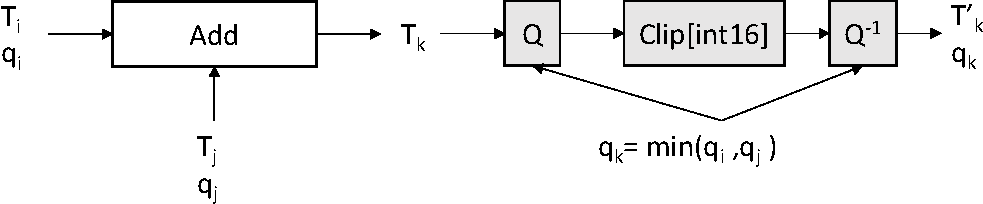
\includegraphics[scale=0.5]{add.pdf}
\caption{Add layer modification}\label{addfig}
\end{figure}

\begin{figure}[p]
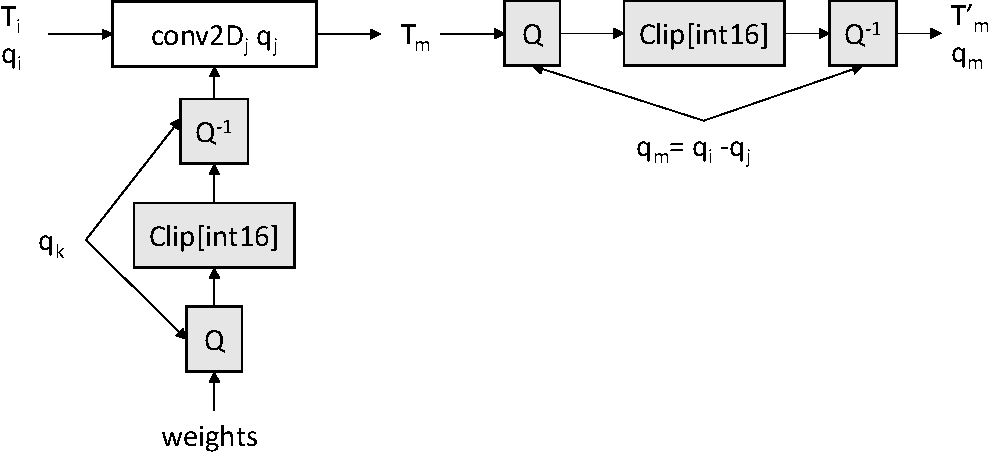
\includegraphics[scale=0.5]{conv2d.pdf}
\caption{Convolution2D layer modification}
\end{figure}

\begin{figure}[p]
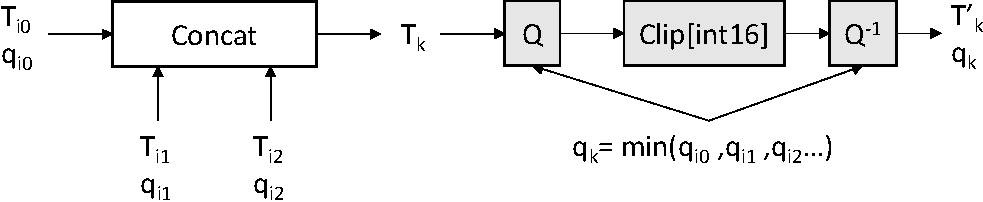
\includegraphics[scale=0.5]{concat.pdf}
\caption{Concatenate layer modification}
\end{figure}

\begin{figure}[p]
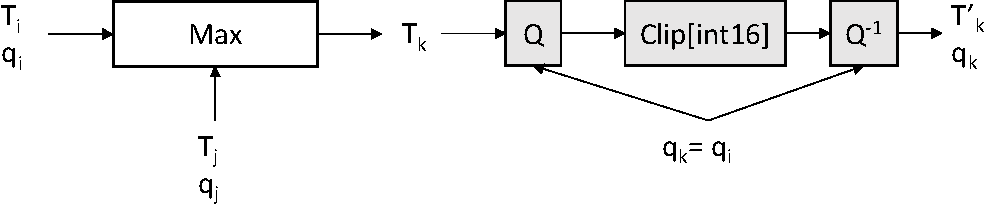
\includegraphics[scale=0.5]{max.pdf}
\caption{Max layer modification}
\end{figure}

\begin{figure}[p]
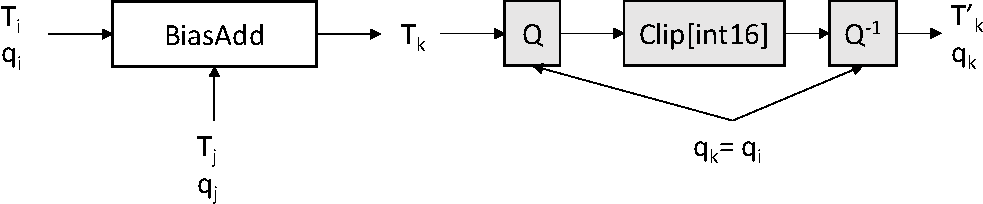
\includegraphics[scale=0.5]{biasadd.pdf}
\caption{BiasAdd layer modification}
\end{figure}

\begin{figure}[p]
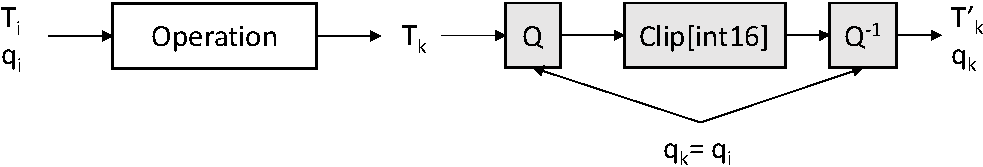
\includegraphics[scale=0.5]{operation.pdf}
\caption{Default modification for other layers}\label{opfig}
\end{figure}


\subsection{Normalization}
In order to get the inputs values without any loss, it is recommended to normalize the data using power of 2. For example, luma samples in the range 0-1023 should be normalized by dividing by 1024 during the float model training. In this case, the integer model uses a quantizer parameter of 10 and uses directly the luma samples.


\section{Other information}
\begin{itemize}
\item {\href{https://jvet-experts.org/doc_end_user/documents/23_Teleconference/wg11/JVET-W0181-v5.zip} AHG11: Small Ad-hoc Deep-Learning Library}
\item \href{https://jvet-experts.org/doc_end_user/documents/25_Teleconference/wg11/JVET-Y0110-v3.zip}{JVET-Y0110: AHG11: Small Ad-hoc Deep-Learning Library (SADL) update}
\item \href{https://jvet-experts.org/doc_end_user/documents/26_Teleconference/wg11/JVET-Z0161-v3.zip}{JVET-Z0161 AhG11: SADL update}
\item{JVET-AA0086 AHG11: Small Ad-hoc Deep-Learning Library (SADL) update}

\end{itemize}
\end{document}
